\documentclass{article}

\usepackage{Paper}
\pdftitle{Frongillo_Moos_EENG_Presentation_Handout}

% === TITLE ===
\title{\textbf{Gravity Energy Storage Systems (GESS) \\ EENG Handout Presentation, HS25}}
\author{Matteo Frongillo, Michael Moos}
\date{\today}

% === TEXT ===
\begin{document}
\newgeometry{
    a4paper,
    total={170mm,257mm},
    left=20mm,
    top=0mm,
    bottom=20mm
}
\hypersetup{citecolor=black}
\maketitle
\linespread{1.2}\selectfont

In Switzerland, potential energy storage is widely used for producing
green energy in the form of pumped hydro plants. Due to the limited
space in cities, Gravity Energy Storage Systems (GESS) are an efficient
alternative for the generation of clean power \parencite{franklin2022}.
In order to make this type of storage possible, the company Energy Vault$^{\textregistered}$
developed the G-VAULT\texttrademark. The principle is simple: energy is stored by using
excess green electricity to lift heavy masses (such as concrete blocks) and later
releases it by lowering them to generate electricity. This process is based on the
conversion between potential and kinetic energy \parencite{energyvault2023}.

\vspace{-0.3cm}
\begin{wrapfigure}{l}{.5\textwidth}
    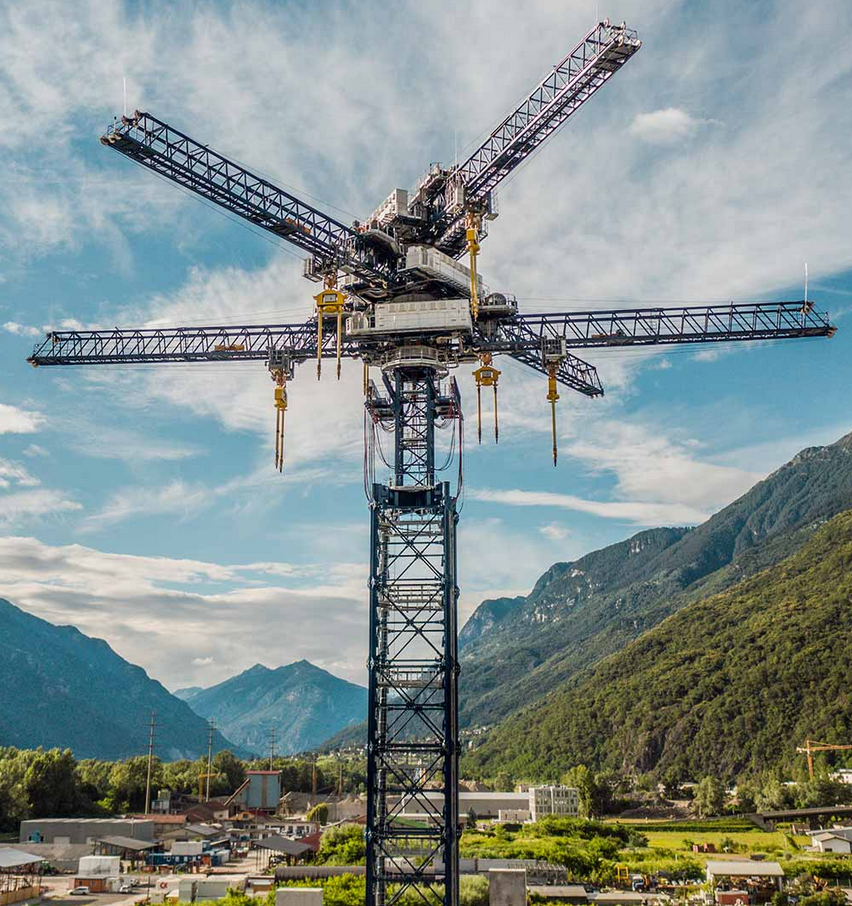
\includegraphics[width=.5\textwidth]{media/EV_prototype.png}
    \caption{Prototype 1 in Arbedo-Castione, Switzerland}
\end{wrapfigure}

\phantom{}

Modern gravity storage systems use large cranes or tower structures
controlled by advanced automation software. When renewable energy
sources like solar or wind produce more electricity than needed, the
system powers electric motors that lift the weights. This principle
of lifting concrete blocks can also be applied to pumping hydro
power, and the fluid will then act as the weight. During times of
high demand, the weights are lowered, and the motors act as
generators, feeding electricity back into the grid.
\wrapfill

\vspace*{-1.5cm}

\begin{wrapfigure}{r}{.4\textwidth}
    \vspace*{-5cm}
    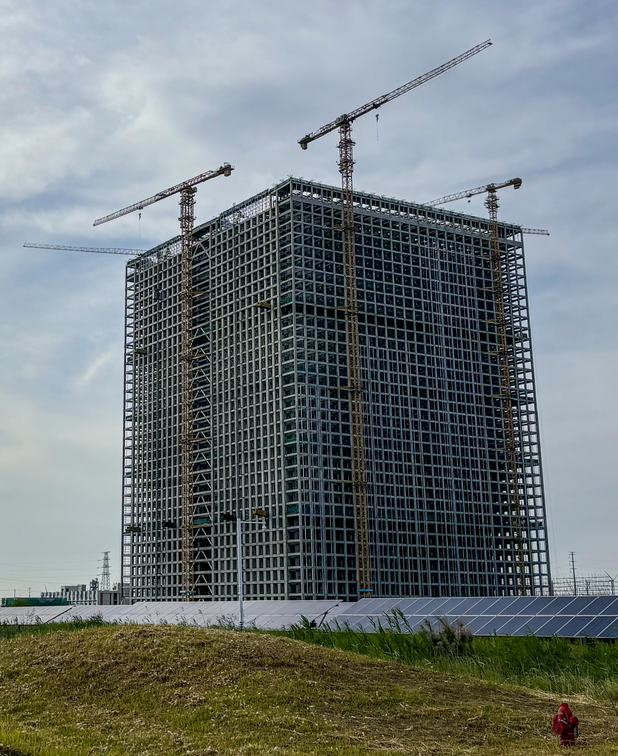
\includegraphics[width=.4\textwidth]{media/EVx.png}
    \caption{EVu\texttrademark\ prototype in China}
\end{wrapfigure}

\vspace*{-0.3cm}
One of the leading companies in this field, Energy Vault, has
demonstrated that such systems can reach high round-trip efficiencies
of around 80\% and long lifespans with minimal environmental impact.
Unlike lithium-ion batteries gravity-based storage does not degrade
over time, requires no rare materials, and poses no fire risk.
Additionally, these systems can be built using local materials
reducing transportation costs and carbon footprint
\parencite{mombelli2020}.
\wrapfill

\vspace*{-1cm}
The main challenges are high initial costs, space requirements,
and energy density compared to chemical batteries. However, as
renewable energy integration grows, gravity storage provides a
scalable and sustainable solution for stabilizing power grids and
ensuring energy availability even when the sun doesn’t shine or the
wind doesn’t blow.

\newpage
\restoregeometry
\section*{Word Bank}
\begin{table}[ht!]
    \renewcommand{\arraystretch}{2}
    \centering
    \begin{tabularx}{\textwidth}{|l|X|}
        \hline
        \textbf{Term} & \textbf{Definition} \\
        \hline
        Potential Energy & Stored energy due to an object’s height or position. \\
        \hline
        Kinetic Energy & Energy released when an object moves or falls. \\
        \hline
        Renewable Energy & Power generated from natural, sustainable sources like wind or solar. \\
        \hline
        Pumped Hydro Storage & Energy storage method using water pumped between two elevations. \\
        \hline
        Gravity Energy Storage (GESS) & A system that lifts heavy masses to store energy and lowers them to release it. \\
        \hline
        Round-Trip Efficiency & The percentage of energy recovered compared to the amount originally stored. \\
        \hline
        Automation Software & Computer programs that control machines automatically for precision and safety. \\
        \hline
        Infrastructure & The physical structures and systems needed for power generation and storage. \\
        \hline
        Energy Density & The amount of energy stored per unit of mass or volume. \\
        \hline
        Mechanical Storage & Energy storage using physical motion instead of chemical reactions. \\
        \hline
        Grid Stability & The reliability and balance of electricity supply in a power network. \\
        \hline
        Sustainability & Using resources responsibly so they remain available for the future. \\
        \hline
        Degradation & The process of losing efficiency or capacity over time. \\
        \hline
        Carbon Footprint & The total greenhouse gas emissions caused directly or indirectly by an activity. \\
        \hline
        Lifespan & The operational duration of a system before replacement or decommissioning. \\
        \hline
        Local Materials & Construction materials sourced regionally to reduce transport and emissions. \\
        \hline
        Energy Conversion & The transformation of one energy form (e.g., electrical) into another (e.g., mechanical). \\
        \hline
        Scalability & The ability of a system to expand while maintaining performance. \\
        \hline
        Decarbonization & Reducing carbon emissions by switching to clean energy technologies. \\
        \hline
        Grid Integration & Connecting renewable or storage systems to the main power grid for coordinated operation. \\
        \hline
    \end{tabularx}
\end{table}

\newpage
\section*{Declarations on the use of AI tools}
\begin{itemize}
    \item ``DeepL'' and ``ChatGPT 5'' have been used as a spell-checker \\
        \url{https://www.deepl.com/}\\
        \url{https://www.chatgpt.com/}
\end{itemize}

\listoffigures

\setlength{\bibitemsep}{1.2\baselineskip}
\printbibliography[title={References}]

\end{document}
